\chapter{引言}
\label{chap:introduction}

\section{异构并行计算}
\label{sec:heterogeneous-parallel-computing}

从计算诞生之初起，许多高价值应用就要求比计算设备所能提供的更多执行速度和
资源。早期应用依靠处理器速度、内存速度和内存容量的提升，来增强应用层面的能力，
例如提高天气预报的及时性、工程结构分析的准确性、计算机生成图形的逼真度，以及
每秒处理的航班预订数或资金转账数。近年来，深度学习等新应用对执行速度和资源的
需求甚至超过了最先进计算设备的供给。这些应用需求在过去五十年中推动了计算设备
能力的快速发展，并且在可预见的未来仍将继续推动这种发展。

以单个中央处理器（central processing unit，CPU）为基础、看起来按照顺序执行指令
的微处理器，例如 Intel 和 AMD 的 x86 处理器，在 20 世纪 80 年代和 90 年代依靠
不断提高的时钟频率和硬件资源，推动了计算应用性能的快速提升和成本的持续下降。
在这二十年的增长期内，单 CPU 微处理器把 GFLOPS（giga，即 $10^9$ 次浮点运算
每秒）带到了桌面计算机，把 TFLOPS（tera，即 $10^{12}$ 次浮点运算每秒）带到了
数据中心。这种对性能改进的不懈追求，使应用软件能够提供更多功能、更好的用户界面
以及更有用的结果。用户一旦习惯了这些改进，就会进一步要求更多改进，从而形成计算
机产业的正向（良性）循环。

然而，由于能耗和散热问题，这种发展势头在 2003 年之后放缓了。这些问题限制了
时钟频率的提升，也限制了单个 CPU 在保持“按顺序执行指令”这一表象的同时、能够在
每个时钟周期内完成的有效工作量。此后，几乎所有微处理器厂商都转向在每个芯片中
使用多个物理 CPU（称为处理器核心）来提高处理能力。在这种模型下，传统 CPU 可以
看作单核 CPU。要从多个处理器核心中获益，用户必须拥有多个指令序列——它们可以来自
同一个应用，也可以来自不同应用——以便在这些处理器核心上同时执行。对于某个应用
而言，要想利用多个处理器核心，就必须把其工作划分为多个能够同时在这些核心上执行
的指令序列。这种从单 CPU 按顺序执行指令转向多核心并行执行多个指令序列的变化，
对软件开发者群体产生了深远影响。

传统上，绝大多数软件应用都是顺序程序；处理器的设计思想源自冯·诺伊曼在 1945 年
发表的奠基性报告 \cite{vonneumann1993}。人们可以借助程序计数器（program counter，
在相关文献中也称 instruction pointer）这一概念，把这些程序的执行理解为沿着程序
代码逐条向前推进。程序计数器保存处理器将要执行的下一条指令的内存地址。应用以
这种逐步顺序方式执行指令所形成的指令执行序列，在相关文献中称为执行线程
（thread of execution），简称线程。本书后文会更正式地定义线程，并广泛使用这一
概念；它的重要性由此可见。

历史上，大多数软件开发者依靠硬件进步——例如更高的时钟频率，以及硬件在幕后同时
执行多条指令——来提高顺序应用的速度。随着新一代处理器问世，同一份软件通常会
自动运行得更快；计算机用户也习惯了每一代微处理器都能让程序运行得更快。然而，
这种预期已经十多年没有成为现实。顺序程序只能运行在某个处理器核心上，而单个核心
在不同代际之间已经不再显著变快。随着性能改进停滞，顺序应用开发者无法再仅靠新
微处理器的推出，为软件加入新的特性和能力，这也削弱了整个计算机产业的增长机会。

相反，在每一代微处理器上仍能持续获得显著性能提升的，是并行软件：多个执行线程
协作完成工作，从而更快地完成任务。并行程序相对于顺序程序的这种优势急剧扩大，
被称为“并发革命”\cite{sutter2005}。并行编程并非新实践。高性能计算领域已经
开发并行程序数十年；这些程序通常运行在规模庞大且价格昂贵的计算机上。只有少数
精英应用能够证明使用这类昂贵计算机是合理的，因此并行编程一度只属于少数应用
开发者。然而，当所有微处理器都变成并行计算机之后，需要以并行程序形式开发的应用
数量急剧增加。软件开发者学习并行编程的需求也随之大幅增长，而这正是本书的重点。

\subsection{多核与众线程路线}

自 2003 年以来，半导体产业主要沿着两条微处理器设计路线发展
\cite{hwu2008}：多核（multi-core）和众线程（many-thread）。多核路线试图在转向
多个核心的同时，保持顺序程序的执行速度。多核处理器最初是双核处理器，之后核心
数量随着每一代半导体工艺不断增加。例如，Intel 和 AMD 的多核服务器微处理器
可以拥有超过 100 个处理器核心；每个核心都是支持乱序执行和多指令发射、实现完整
x86 指令集的处理器，并支持两个硬件线程的超线程技术，目标是最大化顺序程序的
执行速度。另一个例子是 ARM Ampere 多核服务器处理器，最多可拥有 128 个处理器
核心。

相比之下，众线程路线更加关注并行应用的执行吞吐量。众线程路线从大量线程起步，
之后线程数量也随着每一代产品不断增加。近期的代表是 NVIDIA Hopper H100 图形
处理器（graphics processing unit，GPU）：它拥有数十万个线程，这些线程在大量
简单的顺序发射流水线上执行。自 2003 年以来，众线程处理器，尤其是 GPU，一直在
浮点性能竞赛中领先。截至 2022 年，H100 GPU 的峰值浮点吞吐量为：64 位双精度
34 TFLOPS、32 位单精度 67 TFLOPS，以及 16 位半精度 1979 TFLOPS。相比之下，
同年典型服务器级 CPU 的峰值浮点吞吐量只有几 TFLOPS。众线程 GPU 与多核 CPU
之间的峰值浮点计算吞吐量差距在过去几年持续扩大。需要注意的是，这些数字不一定
代表应用速度，而只是芯片中的执行资源在理论上能够支持的原始速度。

多核处理器和众线程处理器之间如此巨大的峰值性能差距，仿佛积累起了很大的“电势”；
最终总会有某种变化发生。我们已经到达了这个时刻。迄今为止，这种巨大的峰值性能
差距已经促使许多应用开发者把软件中计算密集的部分迁移到 GPU 上执行。也许更重要
的是，并行执行能力的大幅提升使深度学习等革命性新应用成为可能；这类应用天然由
计算密集的部分组成。不出意外，这些计算密集部分也正是并行编程的首要目标：工作
越多，就越有机会把工作分配给协作的并行工作者，也就是线程。

为什么众线程 GPU 与多核 CPU 之间会存在如此巨大的峰值性能差距？答案在于这两类
处理器截然不同的基本设计理念，如图 \ref{fig:1-1} 所示。CPU 的设计（图
\ref{fig:1-1} 中的左侧部分）针对顺序代码性能进行了优化。算术单元和操作数数据
传送逻辑经过设计，以尽量降低算术运算的有效延迟，但代价是每个单元占用更多芯片
面积和功耗。较大的片上末级缓存用于捕获频繁访问的数据，把一部分长延迟内存访问
转化为短延迟缓存访问。复杂的分支预测逻辑和执行控制逻辑则用来缓解条件分支指令
带来的延迟。通过降低操作延迟，CPU 硬件降低了每个独立线程的执行延迟。然而，
低延迟算术单元、复杂的操作数传送逻辑、大容量缓存和复杂控制逻辑都会消耗芯片面积
与功耗；这些资源本可以用来提供更多算术执行单元和内存访问通道。这种设计方法通常
称为面向延迟的设计（latency-oriented design）。

另一方面，GPU 的设计理念受到快速增长的电子游戏产业塑造。该产业带来了巨大的
经济压力，要求在高级游戏的每一帧画面中完成海量浮点计算和内存访问。这样的需求
促使 GPU 厂商设法把尽可能多的芯片面积和功耗预算用于浮点计算与内存访问吞吐量。

图形应用每秒需要完成海量浮点计算，例如视点变换和物体渲染，这一点很直观。此外，
每秒进行海量内存访问同样重要，甚至可能更加重要。许多图形应用的速度受限于数据
从内存系统送入处理器、以及从处理器送回内存系统的速率。GPU 必须能够在其 DRAM
（动态随机存取存储器）与图形帧缓冲区之间搬运极大量数据，因为正是这种数据移动
让视频显示对玩家而言丰富而有吸引力。游戏应用通常接受一种较为宽松的内存模型
（即各种系统软件、应用和 I/O 设备对于内存访问应如何工作的共同预期），这也让 GPU
更容易支持对内存进行大规模并行访问。

相比之下，通用处理器必须满足传统操作系统、应用和 I/O 设备提出的要求。这些要求
使并行内存访问更加困难，也使提高内存访问吞吐量——通常称为内存带宽
（memory bandwidth）——更加困难。因此，图形芯片的内存带宽一直约为同时代 CPU
芯片的 10 倍，我们预计在一段时间内 GPU 仍将在内存带宽方面占据优势。

一个重要观察是：从功耗和芯片面积的角度看，降低延迟比提高吞吐量昂贵得多。例如，
把算术单元数量加倍，可以把算术吞吐量加倍，代价大致是芯片面积和功耗加倍；但要
把算术延迟减半，可能需要把电流加倍，芯片面积增加到两倍以上，功耗增加到四倍。
因此，GPU 的主流方案是优化大量线程的执行吞吐量，而不是降低单个线程的延迟。
这种设计方法允许流水化的内存通道和算术操作承受较长延迟，从而节省芯片面积和
功耗。内存访问硬件与算术单元所节省下来的面积和功耗，可以让 GPU 设计者在同一
芯片上放置更多这样的单元，进而提高总体执行吞吐量。图 \ref{fig:1-1} 通过视觉
方式展示了两种设计方法的差异：CPU 设计包含较少但更大的算术单元和较少的内存
通道，而 GPU 设计包含更多但更小的算术单元以及更多内存通道。

\begin{figure}[htbp]
  \centering
  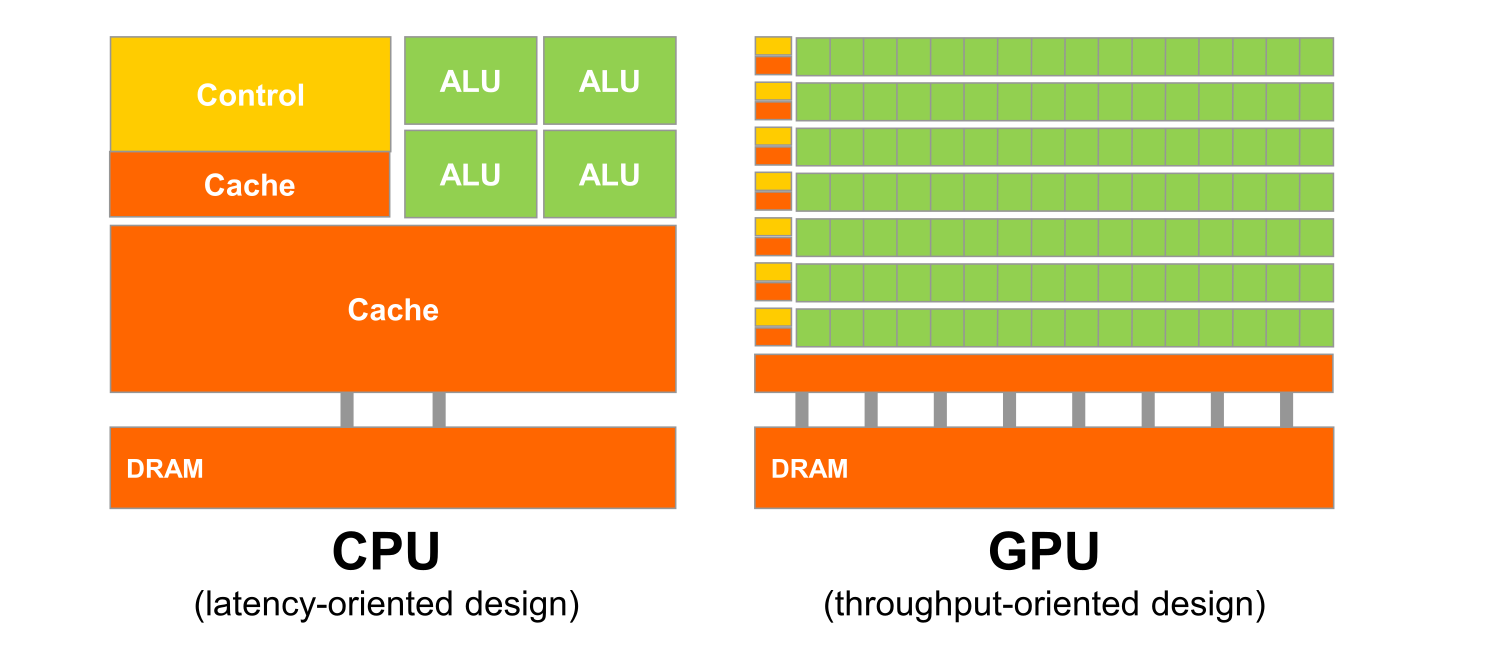
\includegraphics[width=\textwidth]{figs/ch1/1-1.png}
  \caption{CPU 与 GPU 的基本设计理念}
  \label{fig:1-1}
\end{figure}

GPU 应用软件通常需要使用大量并行线程编写。硬件可以利用大量线程，在其中一些
线程等待长延迟内存访问或算术操作时，寻找其他可执行的工作。图 \ref{fig:1-1}
右侧所示的小型缓存用于控制这些应用的带宽需求，使访问相同内存数据的多个线程
不必全部访问 DRAM。这种设计风格通常称为面向吞吐量的设计（throughput-oriented
design）：它允许单个线程可能需要很长时间执行，同时努力最大化大量线程的总体
执行吞吐量。

应当明确，GPU 是为并行、面向吞吐量的计算引擎而设计的；对于 CPU 擅长的某些任务，
GPU 并不会表现良好。对于只有一个或很少线程的程序，具有更低操作延迟的 CPU 可以
获得远高于 GPU 的性能。当程序拥有大量线程时，具有更高执行吞吐量的 GPU 则可以
获得远高于 CPU 的性能。因此，应当预期许多应用会同时使用 CPU 和 GPU：在 CPU
上执行应用的顺序部分，在 GPU 上执行数值密集部分。这正是 NVIDIA 于 2007 年引入
的 CUDA 编程模型被设计用来支持 CPU-GPU 协同执行应用的原因。

应用开发者选择处理器时，速度也不是唯一的决策因素。其他因素甚至可能更加重要。
首先，所选处理器必须在市场上拥有非常广泛的存在，这称为处理器的装机量
（installed base）。原因很简单：只有面对庞大的客户群体，软件开发成本才有充分
的经济合理性。运行在市场占有率很小的处理器上的应用不会拥有广泛的客户群体。
与通用微处理器相比，传统并行计算系统的市场存在极其有限，这一直是一个主要问题。
只有政府和大公司资助的少数精英应用，成功地在这类传统并行计算系统上实现了开发。
众线程 GPU 改变了这一点。由于 GPU 在个人计算机市场上非常流行，其出货量已经达到
数亿。几乎所有台式 PC 和高端笔记本电脑都配有 GPU。如今已有超过 10 亿个支持
CUDA 的 GPU 在使用。如此庞大的市场存在，使这些 GPU 成为对应用开发者具有经济
吸引力的目标。

另一个重要决策因素是实用的形态和易于获得的运行环境。2006 年以前，并行软件应用
主要运行在数据中心服务器或部门级集群上，但这类执行环境往往限制了应用的使用。
例如，在医学成像应用中，基于 64 节点集群机器发表论文没有问题；但实际临床应用
中的 MRI 设备通常由 PC 与专用硬件加速器组合而成。原因很简单：GE 和 Siemens
等制造商不可能向临床场所销售必须配套几机架计算服务器的 MRI 系统，而这样的部署
在高校院系环境中却很常见。事实上，美国国立卫生研究院（NIH）曾有一段时间拒绝
资助并行编程项目，因为他们认为巨型集群机器无法用于临床环境，并行软件的影响会
受到限制。
如今，许多公司已经推出配备 GPU 的 MRI 产品，NIH 也在资助 GPU 计算研究。

在 2006 年以前，图形芯片很难使用，因为程序员必须通过相当于图形 API
（application programming interface，应用程序接口）的函数访问处理单元，也就是
需要使用 OpenGL 或 Direct3D 技术来编程这些芯片。更直白地说，计算必须表达成某种
“绘制像素”的函数，才能在早期 GPU 上执行。这种技术称为 GPGPU，即使用图形处理
器进行通用编程（General Purpose Programming using a Graphics Processing Unit）。
业界更常见的展开是 ``General-Purpose Computing on Graphics Processing Units''；
这里保留原书的表述，并不把两种展开混为一谈。
即使有更高层的编程环境，底层代码仍然需要适配为面向像素绘制的 API。这些 API 限制
了早期 GPU 实际能够编写的应用类型，因此 GPGPU 没有成为普遍的编程现象。尽管如此，
这项技术仍然足够令人兴奋，激励人们完成了一些富有开创性的工作并取得了优秀的研究
成果。

2007 年 CUDA 发布后，一切发生了变化 \cite{cuda2025}。CUDA 带来的并不只是软件变化，
芯片中还增加了额外硬件。NVIDIA 实际上专门划出硅片面积来简化并行编程。在用于并行计算的 G80
及其后继芯片中，GPGPU 程序不再需要经过图形接口，而是由芯片上的新型通用并行
编程接口直接处理 CUDA 程序的请求。这个通用编程接口极大扩展了可以在 GPU 上轻松
开发的应用类型。此外，其他软件层也全部重新设计，使程序员能够使用熟悉的 C/C++
编程工具。

虽然 GPU 是异构并行计算中的重要计算设备类型，但异构计算系统还会把其他重要设备
用作加速器。例如，现场可编程门阵列（field programmable gate array，FPGA）被
广泛用于加速网络应用。本书以 GPU 为学习载体所介绍的技术，同样适用于这类加速器
的编程任务。

\section{为什么需要更高速度或更多并行性？}
\label{sec:why-more-speed}

正如第 \ref{sec:heterogeneous-parallel-computing} 节所述，大规模并行编程的主要
动机，是让应用在未来几代硬件上继续获得速度提升。在“并行模式”和“高级模式与
应用”两部分（第 2、3 部分，即第 7 至第 23 章）中我们会看到，对于适合并行执行
的应用，优秀的 GPU 实现相对于单个 CPU 核心上的顺序执行，可以达到超过
$100\times$ 的加速比。如果应用包含我们所称的“数据并行性”，仅用几个小时的工作
往往就可以获得 $10\times$ 的加速。

有人可能会问，为什么应用会继续要求更高的速度？今天的许多应用似乎已经运行得
足够快了。尽管当今世界有无数计算应用，未来许多令人兴奋的大众市场应用，实际上
就是我们过去称为“超级计算应用”或“超级应用”的东西。

例如，生物学研究界正越来越深入分子层面。显微镜可以说是分子生物学最重要的仪器，
过去主要依靠光学或电子仪器。然而，我们可以借助这些仪器进行的分子级观测存在限制。
把计算模型纳入进来，模拟底层分子活动，并用传统仪器设置边界条件，可以有效地解决
这些限制。借助仿真，我们能够测量比单靠传统仪器所能想象的更多细节，也能检验更多
假设。在可预见的未来，仿真会继续受益于计算速度的提升：在可接受的响应时间内，
能够建模的生物系统规模会扩大，能够模拟的反应时间也会延长。这些增强将对科学和
医学产生巨大影响。

对于视频、音频编码和处理等应用，可以想想我们对数字高清电视（HDTV）相对于旧式
NTSC 电视的满意程度。体验过 HDTV 的细节水平之后，人们很难再回到旧技术。但请
考虑 HDTV 所需的全部处理工作：它是高度并行的过程，三维成像和可视化也一样。未来，
视图合成、把低分辨率视频以高分辨率显示等新功能，将需要电视设备提供更多计算能力。
在消费级产品中，我们正看到越来越多的视频和图像处理应用，用来改善照片和视频的
对焦、光照以及其他关键方面。

更高的计算速度还可以带来更好的用户界面。现代智能手机用户享受着更加自然的交互
界面，高分辨率触摸屏的显示效果足以媲美大屏电视。毫无疑问，未来版本的这类设备
将加入具有三维视角的传感器和显示器、把虚拟空间与物理空间信息结合起来以提高
可用性的应用，以及基于语音和计算机视觉的交互界面；这些功能都需要更高的计算速度。

消费电子游戏中也在发生类似的发展。过去，游戏中的驾驶实际上只是预先安排好的一
组场景：汽车撞上障碍物后，车辆行驶路线并不会改变，只有游戏分数发生变化；车轮
不会弯曲或损坏，无论撞到车轮还是失去一个车轮，驾驶难度都不会改变。随着计算速度
提升，游戏可以基于动态仿真，而不再基于预先安排的场景。未来我们可以体验更多
这样的真实效果：事故会损坏车轮，在线驾驶体验也会逼真得多。准确建模物理现象的
能力已经催生了“数字孪生”概念：物理对象在仿真空间中拥有准确模型，可以以低得多
的成本进行充分的压力测试和劣化预测。对物理效应进行逼真的建模和仿真，通常需要
极其巨大的计算能力。

计算吞吐量大幅提升所带来的新应用中，一个重要例子是基于人工神经网络的深度学习。
尽管神经网络从 20 世纪 70 年代起就一直受到积极研究，但由于训练需要太多带标签
数据和太多计算，它们在实际应用中一度效果不佳。互联网的兴起带来了海量带标签的
图片，GPU 的兴起则带来了计算吞吐量的跃升。结果，自 2012 年以来，基于神经网络
的应用在计算机视觉和自然语言处理领域迅速普及。这种普及彻底改变了计算机视觉和
自然语言处理应用，也推动了自动驾驶汽车和家庭助手设备的快速发展。

上述所有新应用都以不同方式、不同层次模拟和/或表示一个物理的、并发的世界，并且
需要处理极大量数据。面对如此巨大的数据量，大部分计算都可以在数据的不同部分上
并行完成，尽管这些结果最终需要在某个时刻汇合。多数情况下，有效管理数据传送
会对并行应用能够达到的速度产生重大影响。少数每天处理这类应用的专家往往熟悉
相关技术，但绝大多数应用开发者都能从对这些技术更直观的理解和实践性工作知识中
获益。

我们的目标是以直观的方式向应用开发者介绍数据管理技术，而他们的正规教育未必来自
计算机科学或计算机工程。我们还希望提供大量实用代码示例和动手练习，帮助读者
获得真正可工作的知识；这要求有一种既便于并行实现、又支持恰当管理数据传送的
实用编程模型。CUDA 提供了这样的编程模型，并且已经得到庞大开发者社区的充分检验。

\section{加速真实应用}
\label{sec:speeding-up-real-applications}

把应用并行化后，能够期待多大的加速比？计算系统 $A$ 相对于计算系统 $B$ 的应用
加速比，定义为应用在 $B$ 上的执行时间与在 $A$ 上执行同一应用所需时间之比。例如，
某应用在系统 $A$ 上需要 10 秒，在系统 $B$ 上需要 200 秒，那么系统 $A$ 相对于
系统 $B$ 的加速比为
\[
  \frac{200\text{ s}}{10\text{ s}}=20,
\]
即 $20\times$（20 倍）加速。

并行计算系统相对于串行计算系统能够达到的加速比，取决于应用中可以并行化的部分。
例如，如果应用执行时间中可并行部分占 30\%，即使把这部分加速 $100\times$，应用
总执行时间也最多只能减少 29.7\%。换言之，整个应用的加速比只有
\[
  \frac{1}{1-0.297}\approx 1.42\times.
\]
事实上，即使并行部分获得无限大的加速，也只能削减 30\% 的执行时间，最高加速比
不超过约 $1.43\times$。另一方面，如果执行时间的 99\% 都属于并行部分，那么将
并行部分加速 $100\times$ 后，应用执行时间会降至原来的 1.99\%，整个应用可以获得
$50\times$ 加速。因此，要让大规模并行处理器有效加速应用，应用执行时间的绝大
部分必须位于并行部分。并行执行所能达到的加速水平会受到应用可并行部分大小的
严重限制，这一事实称为阿姆达尔定律（Amdahl's Law）\cite{amdahl2013}。

研究人员已经在某些应用上取得超过 $100\times$ 的加速。然而，这通常只有在进行
大量优化和调优之后才可能实现，而且往往还需要改进算法，使应用工作量的
$99.9\%$ 以上处于并行部分。

应用能够达到的加速水平还取决于从内存读取数据以及向内存写入数据的速度。在实践中，
直接对应用进行并行化往往会使内存（DRAM）带宽达到饱和，结果只能获得约
$10\times$ 加速。诀窍在于设法绕过内存带宽限制：通过某种变换利用 GPU 上的专用
片上内存，大幅减少对 DRAM 的访问。不过，代码还需要继续优化，以应对片上内存
容量有限等限制。本书的一个重要目标，就是帮助读者充分理解这些优化方法并熟练
掌握它们。

请记住，相对于单核 CPU 执行所得到的加速水平，也可能反映 CPU 是否适合该应用。
在某些应用中，CPU 的表现非常好，因此很难再用 GPU 提升性能。大多数应用都有
一些部分更适合由 CPU 执行。必须给 CPU 一个公平的机会，并确保代码编写方式能够
让 GPU 与 CPU 执行互补，从而正确利用 CPU/GPU 组合的异构并行计算能力。如今，
结合多核 CPU 和众核 GPU 的大众市场计算系统，已经把万亿次级（terascale）计算
带到了桌面，把百亿亿次级（exascale）计算带到了集群。

图 \ref{fig:1-2} 展示了典型应用的主要组成部分。真实应用的大量代码往往是顺序的。
图中将这些顺序部分画成桃子的“果核区域”：试图对这些部分应用并行计算技术，就像
咬桃核一样——感觉并不好！这些部分很难并行化。CPU 往往能够很好地处理它们。好
消息是，尽管这些部分可能占据大量代码，却往往只占超级应用执行时间的一小部分。

接下来是我们所谓的“桃肉区域”。这些部分容易并行化，早期图形应用也是如此。在
异构计算系统中进行并行编程，可以大幅提升这类应用的速度。如图 \ref{fig:1-2}
所示，早期 GPGPU 编程接口只覆盖桃肉区域的一小部分，这类似于只能覆盖最令人
兴奋的应用中的一小部分。我们将看到，CUDA 编程接口的设计目标是覆盖更多令人
兴奋的应用“桃肉”。并行编程模型及其底层硬件仍在快速演进，以便高效并行化应用中
越来越大的部分。

\begin{figure}[htbp]
  \centering
  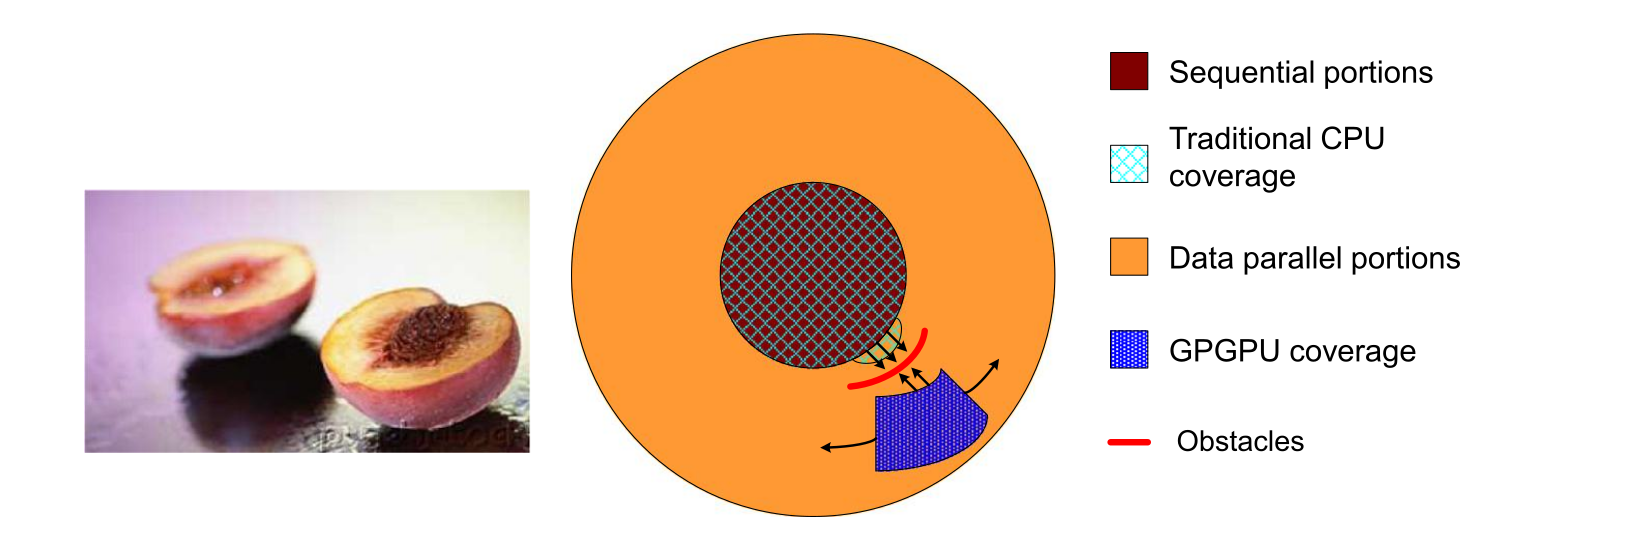
\includegraphics[width=\textwidth]{figs/ch1/1-2.png}
  \caption{顺序部分与数据并行部分的应用结构}
  \label{fig:1-2}
\end{figure}

\section{并行编程中的挑战}
\label{sec:parallel-programming-challenges}

并行编程为什么困难？有人曾说过：如果你不在乎性能，并行编程非常容易；你甚至
可以在一小时内写出并行程序。但如果不在乎性能，又何必编写并行程序呢？

本书讨论如何在并行编程中实现高性能所面临的几个挑战。首先，设计出与顺序算法
具有相同算法（计算）复杂度的并行算法，可能相当困难。许多并行算法与对应的顺序
算法执行相同数量的工作。然而，有些并行算法会做更多工作；事实上，有时它们会
多做如此多工作，以至于在大规模输入数据集上最终运行得更慢。这尤其令人担忧，
因为快速处理大规模输入数据集正是并行编程的重要动机。

例如，许多现实问题最自然的描述方式是数学递推式。把这些问题并行化，通常需要
以反直觉的方式思考问题，执行时也可能需要重复工作。有一些重要的算法原语，例如
前缀和（prefix sum）或扫描（scan），可以帮助我们把问题的顺序递归形式转换为
更适合并行的形式。第 11 章将更正式地介绍工作效率（work efficiency）概念，并
借助前缀和等重要并行模式，说明如何设计具有与对应顺序算法相同计算复杂度的并行
算法，以及其中涉及的方法和权衡。

第二，许多应用的执行速度受内存访问延迟和/或吞吐量限制。我们把这类应用称为
内存受限（memory-bound）应用，以区别于计算受限（compute-bound）应用；后者受
硬件执行算术运算的速率限制。要让内存受限应用实现高性能并行执行，通常需要提高
内存访问速度的方法。第 5 章和第 6 章将介绍内存访问优化技术，并在多章并行模式
与应用中应用这些技术。

第三，相比对应的顺序程序，并行程序的执行速度通常对输入数据特征更加敏感。许多
现实应用必须处理特征变化很大的输入，例如不规则或不可预测的数据规模，以及不
均匀的数据分布。这些规模和分布上的变化，可能导致分配给并行线程的工作量不均，
并显著降低并行执行的有效性。并行程序的性能有时会随这些特征发生剧烈变化。我们
将在介绍并行模式和应用的章节中，介绍使数据分布更加规整，或针对数据特征调整
线程工作分配的技术，以应对这些挑战。

第四，有些应用可以并行化，而且不同线程之间几乎不需要协作。这些应用通常称为
易并行应用（embarrassingly parallel）。另一方面，另一些应用要求线程彼此协作，
这就需要使用屏障或原子操作等同步操作。同步操作会给应用带来开销，因为线程常常
需要等待其他线程，而不是执行有用工作。本书将始终讨论降低这种同步开销的各种
策略。

幸运的是，研究人员过去已经解决了其中许多挑战。不同应用领域之间还存在共同模式，
使我们能够把一个领域中得到的解决方案应用到其他领域。这正是本书选择在重要并行
计算模式和应用的语境中介绍应对这些挑战的关键技术的主要原因。

\section{相关并行编程接口}
\label{sec:related-parallel-interfaces}

过去几十年间，人们已经开发出许多并行编程语言和模型
\cite{mattson2004}。应用最广泛的包括：用于共享内存多处理器系统的 OpenMP
\cite{openmp2025}，以及用于可扩展集群计算的消息传递接口（Message Passing
Interface，MPI）\cite{mpi1994}。二者都已经成为由主要计算机厂商支持的标准化
编程接口。

一个 OpenMP 实现由编译器和运行时系统组成。程序员向 OpenMP 编译器指定有关循环
的指令（directive）和编译提示（pragma）。借助这些指令和提示，OpenMP 编译器
生成并行代码。运行时系统通过管理并行线程和资源，支持并行代码的执行。OpenMP
最初为 CPU 执行设计，后来扩展到支持 GPU 执行。OpenMP 的主要优点是，它提供
编译器自动化和运行时支持，从而把许多并行编程细节抽象掉。这样的自动化和抽象，
有助于让应用代码在不同厂商生产的系统之间，以及同一厂商不同代际的系统之间，
实现更好的可移植性。我们把这一性质称为性能可移植性（performance portability）。
不过，要有效地使用 OpenMP，程序员仍然需要理解涉及的全部并行编程概念。由于
CUDA 让程序员能够显式控制这些并行编程细节，因此即使读者打算把 OpenMP 作为
主要编程接口，CUDA 也是很好的学习载体。此外，根据我们的经验，OpenMP 编译器
仍在不断发展和改进。许多程序员可能仍需在 OpenMP 编译器能力不足的部分使用
CUDA 风格的接口。

MPI 是一种编程接口：集群中的计算节点不共享内存，所有数据共享和交互都必须通过
显式消息传递完成。MPI 已广泛用于高性能计算（high-performance computing，HPC）。
使用 MPI 编写的应用已经在超过 100,000 个节点的集群计算系统上成功运行。如今，
许多 HPC 集群采用异构 CPU/GPU 节点。由于计算节点之间没有共享内存，把应用移植
到 MPI 可能需要相当大的工作量。程序员需要进行域分解，把输入和输出数据划分到
各个节点上；还需要根据域分解结果调用消息发送和接收函数，管理节点之间的数据
交换。

另一方面，CUDA 为 GPU 内部的并行执行提供了共享内存，可以解决这一困难。CUDA
适合节点内部的编程，但大多数应用开发者仍需要使用 MPI 一类的接口来编程集群
层级。随着 MPI 本身逐渐具备 CUDA 感知能力，以及 NCCL 和 NVSHMEM 等其他 API
不断提供支持，CUDA 的多 GPU 编程能力也在增强。因此，在使用多 GPU 节点的现代
计算集群中，并行程序员必须理解如何在 MPI 等多 GPU 编程模型的语境下进行 CUDA
编程；第 23 章将介绍这一内容。

2009 年，包括 Apple、Intel、AMD/ATI 和 NVIDIA 在内的多个产业参与者共同开发了
一种标准化编程模型，称为开放计算语言（Open Computing Language，OpenCL）
\cite{opencl2008}。原书正文将其写作 ``Open Compute Language''；译文采用 OpenCL
的官方展开。与 CUDA 类似，OpenCL 编程模型定义了语言扩展和运行时 API，
允许程序员管理大规模并行处理器中的并行性和数据传送。与 CUDA 相比，OpenCL
更多依赖 API，而较少依赖语言扩展。这样，厂商就可以快速调整现有编译器和工具，
以处理 OpenCL 程序。

OpenCL 是一种标准化编程模型：使用 OpenCL 开发的应用，无需修改，就能在所有
支持 OpenCL 语言扩展和 API 的处理器上正确运行。不过，要在新的处理器上获得
高性能，通常仍然需要修改应用。熟悉 OpenCL 和 CUDA 的读者会知道，二者的关键
概念和特性非常相似。也就是说，CUDA 程序员只需很少努力就能学会 OpenCL 编程。
更重要的是，使用 CUDA 学到的几乎所有技术，都可以轻松应用于 OpenCL 编程。

\section{总体目标}
\label{sec:overarching-goals}

我们的首要目标是教会读者如何编程大规模并行处理器，以实现高性能。因此，本书
很大一部分内容都致力于开发高性能并行代码的技术。我们的方法不要求读者具备
大量硬件专业知识；不过，读者需要对并行硬件架构有良好的概念性理解，才能推理
代码的性能行为。因此，我们会用一些篇幅帮助读者直观理解基本硬件架构特征，并用
大量篇幅介绍开发高性能并行程序的技术。特别是，我们将重点讨论计算思维
（computational thinking）\cite{wing2006} 技术，使读者能够用适合在大规模并行
处理器上高性能执行的方式思考问题。

在大多数处理器上进行高性能并行编程，都需要了解硬件的工作方式。要构建工具和
机器，使程序员不必了解这些知识就能开发高性能代码，可能还需要很多年。即使有了
这样的工具，我们也怀疑了解硬件的程序员会比不了解硬件的人更有效地使用它们。
因此，第 4 章将介绍 GPU 架构的基础；在讨论高性能并行编程技术时，我们还会讨论
更加专门的架构概念。

我们的第二个目标是教授如何编写功能正确且可靠的并行程序；这是并行计算中
一个微妙的问题。曾经开发过并行系统的人都知道，实现初始性能还不够，真正的挑战
是以一种能够调试代码并支持用户的方式实现性能。CUDA 编程模型鼓励使用简单形式
的屏障同步、原子性和内存一致性来管理并行性。此外，它还提供了一组强大的工具，
不仅可以调试功能问题，也可以定位性能瓶颈。

我们的第三个目标是让程序能够跨越未来的硬件代际进行扩展：探索并行编程方法，使
未来更加并行的机器能够比今天的机器更快地运行代码。我们希望帮助读者掌握并行
编程，使程序能够扩展到新一代机器的性能水平。实现这种可扩展性的关键，是使内存
数据访问更加规整和局部化，从而尽量减少关键资源的消耗以及更新数据结构时发生的
冲突。因此，开发高性能并行代码的技术，对保证应用在未来的可扩展性同样重要。

要实现这些目标，需要大量技术知识，因此本书会介绍不少并行编程原则和模式
\cite{mattson2004}。我们不会孤立地教授这些原则和模式，而是把它们放在有用应用
的并行化语境中来讲授。当然，我们无法覆盖全部原则和模式，所以选择了最有用且
经过充分验证的技术进行详细介绍。事实上，本版显著增加了关于并行模式和应用的
章节。现在，让我们快速概览本书其余内容。

\section{本书的组织结构}
\label{sec:book-organization}

本书分为三部分。第 1 部分介绍并行编程、数据并行、GPU 以及性能优化的基本概念。
这些基础章节为读者成为 GPU 程序员提供必要的知识和技能。第 2 部分介绍基本的
并行模式，第 3 部分介绍更高级的并行模式和应用。这两部分会应用第一部分所学的
知识和技能，也会在需要时引入其他 GPU 架构特性和优化技术。

第 1 部分“基础概念”包括第 2 至第 6 章。第 2 章介绍数据并行和 CUDA 编程模型，
并假设读者此前有 C++ 编程经验。它首先把 CUDA 介绍为 C++ 的一个简单而小型的
扩展，用于支持异构 CPU/GPU 计算以及广泛使用的单程序多数据（Single Program
Multiple Data，SPMD）并行编程模型。随后，本章介绍以下思考过程：

\begin{enumerate}
  \item 识别应用程序中需要并行化的部分；
  \item 隔离并行代码将使用的数据，并通过 API 函数在并行计算设备上分配内存；
  \item 通过 API 函数把数据传送到并行计算设备；
  \item 把并行部分开发为由并行线程执行的内核函数；
  \item 启动内核函数，让并行线程执行它；
  \item 最终通过 API 函数调用把数据传回主机处理器。
\end{enumerate}

我们使用向量加法这一贯穿示例来说明这些概念。第 2 章的目标，是让读者掌握足够
的 CUDA 编程模型概念，以便编写简单的并行 CUDA 程序；同时，它也涵盖了基于任何
并行编程接口开发并行应用所需的若干基本技能。

第 3 章进一步介绍 CUDA 的并行执行模型，尤其是它如何处理多维数据以及多维线程
组织方式。本章提供关于线程创建、组织、资源绑定和数据绑定的足够洞见，使读者
能够使用 CUDA 实现复杂计算。

第 4 章介绍 GPU 计算架构，重点讨论计算核心如何组织，以及线程如何被调度到这些
核心上执行。本章还讨论各种架构因素及其对 GPU 上运行代码性能的影响，包括透明
可扩展性、SIMD 执行与控制分歧、多线程与延迟容忍度，以及占用率（occupancy）
等概念。

第 5 章在第 4 章基础上讨论 GPU 的内存架构，以及可用于保存 CUDA 变量、管理数据
传送和提高程序执行速度的特殊内存。本章介绍分配和使用这些内存的 CUDA 语言特性。
恰当地使用这些内存，可以大幅提高数据访问吞吐量，并帮助缓解内存系统中的流量
拥塞。

第 6 章介绍当前 CUDA 硬件中的若干重要性能因素，尤其是理想的线程执行模式和
内存访问模式。这些细节构成了程序员推理计算和数据组织决策后果的概念基础。本章
最后给出 GPU 程序员经常使用的常见优化策略检查清单，用于优化各种计算模式。
在本书接下来的两部分中，我们会反复使用这份检查清单来优化不同的并行模式和应用。

第 2 部分“基本并行模式”包括第 7 至第 15 章。第 7 章介绍卷积，这是一种常用的
并行计算模式，源于数字信号处理和计算机视觉，并且需要仔细管理数据访问局部性。
我们还借助该模式介绍现代 GPU 中的常量内存和缓存。第 8 章介绍与卷积相似的
模板计算，但它源于求解微分方程，并具有为数据访问局部性进一步优化提供独特机会
的特征。本章还用来介绍线程与数据的三维组织，并展示第 6 章中针对线程粒度的优化
方法。

第 9 章讨论直方图，这是一种广泛用于统计数据分析和大规模数据集模式识别的模式。
我们还借助该模式介绍原子操作，用于协调对共享数据的并发更新；并介绍私有化
（privatization）优化，以降低这些操作的开销。第 10 章介绍归约树模式，用于概括
一组输入数据；同时用它展示控制分歧和过多屏障同步对性能的影响，以及减轻这些影响
的技术。第 11 章介绍前缀和或扫描，这是一种重要的并行计算模式，可以把本质上
顺序的计算转换为并行计算；我们也借此介绍并行算法中的工作效率概念。第 12 章
以两种形式介绍过滤模式：不稳定过滤（允许改变被过滤元素的原始顺序）和稳定过滤
（必须保留原始顺序）。不稳定过滤用于展示线程如何协作以减少原子操作，稳定过滤
则展示第 11 章介绍的扫描模式的一个重要应用。第 13 章介绍并行归并，这是分治式
工作划分策略中广泛使用的模式；本章还介绍动态输入数据识别与组织。最后，第
14 章介绍 GPU 上的排序，涵盖三种并行排序算法：奇偶排序、归并排序（依赖第 13
章的归并模式）以及基数排序（依赖第 11 章介绍的扫描模式）。第 15 章更深入地
重新讨论矩阵乘法，应用第 6 章检查清单中的大量高级优化方法。

\footnote{原书此处把基数排序所依赖的扫描模式标为 Chapter 14；按本书目录和上下文，
应为 Chapter 11。译文按语境更正，并保留此译者注。}

第 3 部分“高级并行模式与应用”在精神上与第 2 部分类似，但所涵盖的模式更加复杂，
通常也包含更多应用背景。因此，这些章节较少侧重介绍新技术或新特性，而更多关注
特定应用的考量。对于每个应用，我们首先识别构造并行执行的不同方式，然后分析
每种方式的优点和缺点，接着逐步进行实现高性能所需的代码变换。这些章节帮助读者
把前面章节的全部材料结合起来，并为读者承担自己的应用开发项目提供支持。

第 3 部分包括第 16 至第 23 章。第 16 章以图处理中的经典 Floyd--Warshall 算法
和基因组序列比对中的 Smith--Waterman 算法为贯穿示例，展示动态规划和波前并行。
第 17 章介绍稀疏矩阵计算，这一技术广泛用于处理极大规模数据集。本章向读者介绍
重新排列数据以实现更高效并行访问的概念，包括数据压缩、填充、排序、转置和规整化。
第 18 章介绍图算法，以及如何在 GPU 编程中高效实现图搜索。本章给出并行化图算法
的多种策略，并讨论图结构如何影响最佳算法的选择；这些策略建立在直方图和归并等
更基本的模式之上。

第 19 章和第 20 章讨论深度学习，它已经成为 GPU 计算中极其重要的领域。第 19 章
介绍卷积神经网络的高效实现，利用分块等技术和卷积等模式。第 20 章介绍大语言
模型，并讨论在 GPU 上训练和推理这些模型的先进优化方法，例如 KV 缓存和批处理。
第 21 章讨论静电势图计算，以及如何利用从散布到聚集的变换来增强并行性、降低
同步开销。

第 22 章介绍计算思维，即以更适合高性能计算的方式构造和求解计算问题的艺术。
本章讨论如何组织程序的计算任务，使其能够并行执行。我们首先讨论把抽象的、特定
于科学问题的概念转化为计算任务的过程；无论开发串行还是并行应用，这是生成高质量
应用软件的重要第一步。随后，我们讨论并行算法结构及其对应用性能的影响，并以
CUDA 性能调优经验为基础。虽然我们不深入介绍这些并行编程风格的实现细节，但希望
读者能够凭借本书打下的基础，学会使用其中任何一种风格编程。本章最后区分并行化
计算的两种广泛策略：以输入为中心和以输出为中心，并回到书中介绍的模式与应用，
回顾性地研究每种模式和应用所采用的策略。

第 3 部分的最后一章，即第 23 章，介绍异构集群上的 CUDA 编程，其中每个计算节点
都包含 CPU 和 GPU。我们讨论如何在 CUDA 的配合下使用 MPI、NCCL 和 NVSHMEM
三种不同编程模型，把计算分配到集群中的多个 GPU，同时降低通信开销。

虽然本书各章都以 CUDA 为基础，但它们帮助读者建立的是一般并行编程的基础。我们
相信，人类从具体示例中学习效果最好：也就是说，必须首先在某个特定编程模型的
语境中学习概念；该模型为我们把知识推广到其他编程模型提供坚实立足点。在推广
过程中，我们可以借助从 CUDA 示例中获得的具体经验。深入体验 CUDA 也能帮助我们
形成成熟的理解，从而学习那些甚至可能与 CUDA 模型无关的概念。

第 24 章将对大规模并行编程作总结并展望未来。我们首先重新审视本书目标，总结各章
如何共同帮助实现这些目标；然后预测快速发展的大规模并行计算会使其成为未来十年
最令人兴奋的领域之一。

\begin{chapterbibliography}{10}

\bibitem{vonneumann1993}
J. von Neumann.
First draft of a report on the EDVAC.
\emph{IEEE Annals of the History of Computing}, 15(4), 1993, 27--75.

\bibitem{sutter2005}
H. Sutter and J. Larus.
Software and the concurrency revolution: leveraging the full power of multicore
processors demands new tools and new thinking from the software industry.
\emph{ACM Queue}, 3(7), 2005, 54--62.

\bibitem{hwu2008}
W.-M. Hwu, K. Keutzer, and T. G. Mattson.
The concurrency challenge.
\emph{IEEE Design \& Test of Computers}, 25(4), 2008, 312--320.

\bibitem{cuda2025}
NVIDIA.
\emph{CUDA C++ Programming Guide}, Release 13.0, 2025.
\url{https://docs.nvidia.com/cuda/cuda-c-programming-guide}.

\bibitem{amdahl2013}
G. M. Amdahl.
Computer architecture and Amdahl's law.
\emph{Computer}, 46(12), 2013, 38--46.

\bibitem{mattson2004}
T. G. Mattson, B. Sanders, and B. Massingill.
\emph{Patterns for Parallel Programming}.
Pearson Education, 2004.

\bibitem{openmp2025}
OpenMP.org.
\emph{OpenMP: The OpenMP API Specification for Parallel Programming}, 2025.
\url{https://www.openmp.org}.

\bibitem{mpi1994}
MPI Forum.
\emph{MPI: A Message-Passing Interface Standard}, 1994.

\bibitem{opencl2008}
Khronos OpenCL Working Group.
\emph{The OpenCL Specification}, Version 1.0, 2008.

\bibitem{wing2006}
J. M. Wing.
Computational thinking.
\emph{Communications of the ACM}, 49(3), 2006, 33--35.

\end{chapterbibliography}
